\begin{figure}[hbt!]
    \begin{subfigure}[b]{0.5\textwidth}
        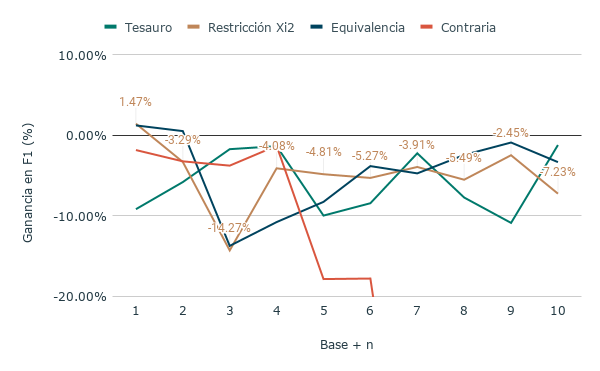
\includegraphics[width=\textwidth]{sections/figures/bi_LSTMAnox.png}
        \caption{Bi-LSTM}
    \end{subfigure}
    \hfill
    \begin{subfigure}[b]{0.5\textwidth}
        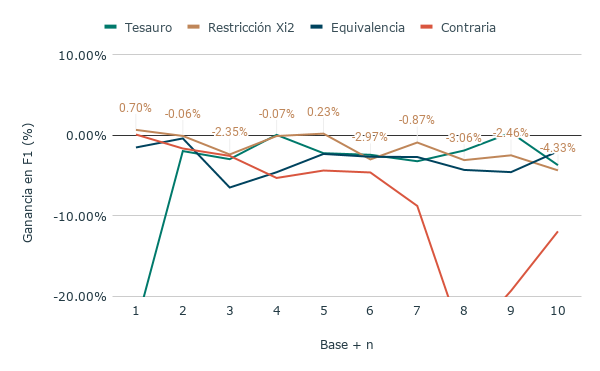
\includegraphics[width=\textwidth]{sections/figures/CNNAnox.png}
        \caption{CNN}
    \end{subfigure}
    \hfill
    
    

    \begin{subfigure}[b]{0.5\textwidth}
        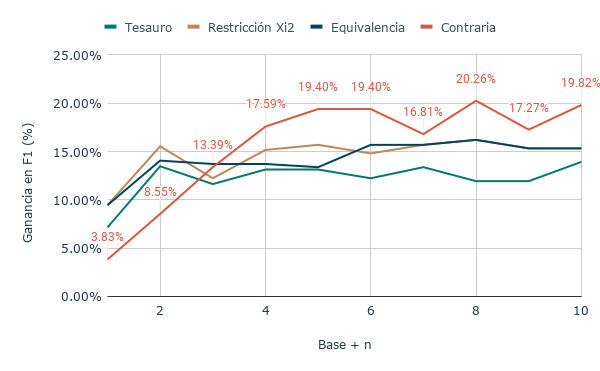
\includegraphics[width=\textwidth]{sections/figures/SVMAnox.png}
        \caption{SVM}
    \end{subfigure}
    \begin{subfigure}[b]{0.5\textwidth}
        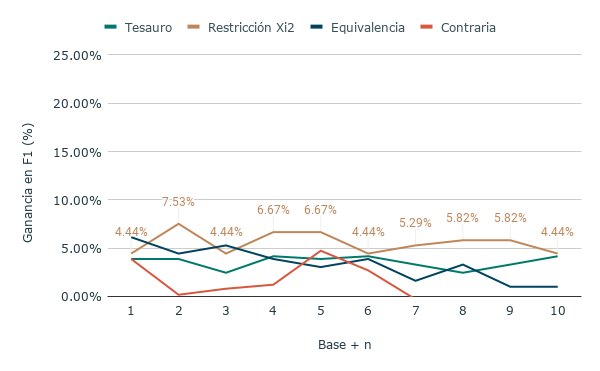
\includegraphics[width=\textwidth]{sections/figures/SVM-CAnox.png}
        \caption{SVM-C}
    \end{subfigure}
    
    \caption{Relación entre el aumento del conjunto de datos y la ganancia en F1 para el conjunto \textit{Anorexia}.}
    \label{fig:aumento_n_anorexia}
\end{figure}